\chapter{Phân tích hệ thống thông tin}
\section{Bài toán và các hoạt động nghiệp vụ}
Từ các luồng thực sự được cài đặt, bài toán phần mềm là tập trung hóa dữ liệu bán lẻ thời trang và hỗ trợ chăm sóc khách hàng. Nhân viên tạo/tra cứu sản phẩm, biến thể và tồn kho; xử lý đơn trực tuyến hoặc tại quầy; theo dõi phương thức/trạng thái thanh toán; quản trị viên phân quyền người dùng; bộ phận CRM duy trì hồ sơ khách, tiếp nhận phản hồi, triển khai khảo sát và trao đổi qua chat.

Khi khách tạo đơn, API kiểm tra thông tin đơn, tồn kho, khuyến mãi và điểm thưởng rồi lưu order, chi tiết và payment. Chuyển khoản QR demo tạo liên kết có token ngẫu nhiên hết hạn sau 15 phút; đây là luồng mô phỏng, không xác minh giao dịch ngân hàng. Nhân viên vẫn có thể xác nhận trạng thái thanh toán thủ công. Sự kiện nghiệp vụ được ghi qua outbox, relay chuyển lên Kafka, consumer lưu bản chiếu sự kiện trong PostgreSQL.

Quy trình CRM gồm quản lý hồ sơ và thuộc tính khách, liên kết sở thích, phân nhóm theo hạng/độ tuổi/giới tính, ghi phản hồi, tạo câu hỏi khảo sát, mời khách, nhận câu trả lời và xem thống kê. Khách tự đăng ký/đăng nhập, cập nhật hồ sơ, gửi đánh giá, thực hiện khảo sát, theo dõi đơn và liên hệ CSKH.

Các hoạt động nghiệp vụ được triển khai có thể tóm tắt theo trình tự sau:
\begin{enumerate}
\item \textbf{Quản lý catalog và nhập hàng:} người có quyền tạo/cập nhật sản phẩm, danh mục, biến thể size/màu, SKU, giá nhập, giá bán và nhà cung cấp. Khi lập phiếu nhập, người dùng chọn nhà cung cấp, biến thể, số lượng và giá nhập mỗi đơn vị; API ghi phiếu cùng dòng chi tiết và cộng lượng tồn. Phiếu xuất ghi số lượng, đơn giá ghi nhận và trừ tồn; API từ chối số lượng vượt tồn. Các thao tác nằm tại \texttt{client/src/views/InventoryManagementView.jsx}, \texttt{server/src/routes/inventory.js} và \texttt{server/src/domain/inventory.js}.
\item \textbf{Bán hàng:} khách duyệt catalog, đưa sản phẩm vào giỏ, chọn địa chỉ giao hàng và gửi đơn; nhân viên có thể tạo đơn tại quầy. API xác thực từng biến thể, giá, số lượng, khuyến mãi và điểm thưởng, lưu đơn/chi tiết/thanh toán trong PostgreSQL và điều chỉnh tồn theo luồng nghiệp vụ. Nhân viên cập nhật trạng thái đơn và thanh toán theo quyền.
\item \textbf{Chăm sóc khách hàng:} khách đăng ký và cập nhật hồ sơ, sở thích; nhân viên CRM tra cứu hồ sơ, tiếp nhận đánh giá, trả lời/cập nhật trạng thái, tạo khảo sát và xem kết quả. Khách chỉ xem và thao tác trên hồ sơ, đơn, phản hồi, khảo sát, hội thoại của mình theo các route được bảo vệ.
\item \textbf{Quản trị và nhân sự:} ADMIN tạo tài khoản, đổi role, khóa/mở và xóa tài khoản khi đáp ứng ràng buộc an toàn. Quản lý nhân sự quản lý hồ sơ nhân viên và xem thống kê theo trạng thái, chức vụ, ngày vào làm. Chưa có bản ghi công việc, chấm công, lương hay nghỉ phép.
\item \textbf{Báo cáo và sự kiện:} người dùng có quyền xem đúng nhóm báo cáo; bảng/biểu đồ lọc theo khoảng ngày và có thể xuất CSV. Sự kiện nghiệp vụ được ghi vào outbox cùng giao dịch, sau đó relay chuyển tới Kafka và consumer ghi dữ liệu event mirror theo mã sự kiện.
\end{enumerate}

Các hạn chế có căn cứ trong source: không có HRM chấm công/tính lương hoặc yêu cầu nghỉ; không có bảng/công việc (task) hay MRP/BOM/sản xuất; chưa tích hợp xác nhận thanh toán từ ngân hàng; không có bằng chứng CRM automation hay gửi thông báo marketing tự động ngoài luồng khảo sát/voucher được cài đặt. Repository không có kết quả đo tải; không kết luận hệ thống đã đạt SLA.

\section{Sơ đồ chức năng}
\IfFileExists{diagrams/01-chuc-nang.pdf}{\begin{figure}[htbp]\centering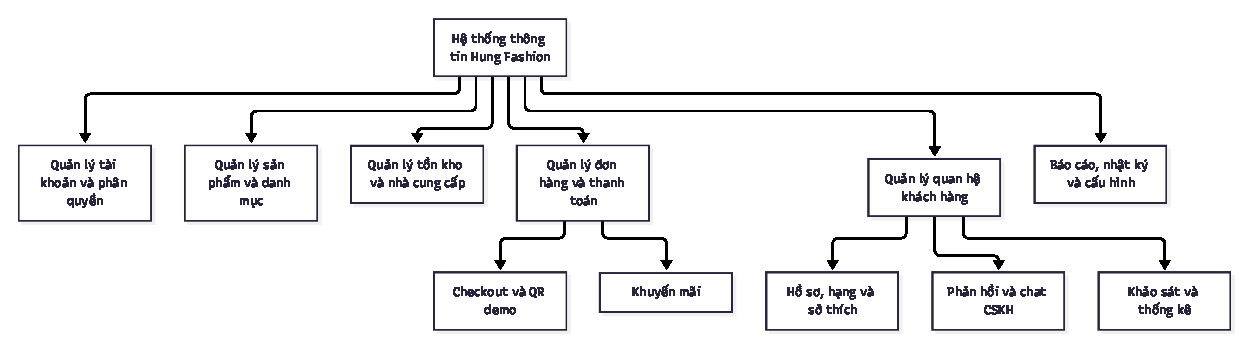
\includegraphics[width=0.88\textwidth]{diagrams/01-chuc-nang.pdf}\caption{Sơ đồ phân rã chức năng theo module đã cài đặt}\label{fig:functions}\end{figure}}{\begin{figure}[htbp]\centering\fbox{\parbox[c][2cm][c]{0.82\textwidth}{\centering Cần kết xuất Mermaid từ \texttt{diagrams/01-chuc-nang.mmd}}}\caption{Sơ đồ phân rã chức năng theo module đã cài đặt}\label{fig:functions}\end{figure}}

\FloatBarrier
\clearpage
\Needspace{0.72\textheight}
\section{Sơ đồ ngữ cảnh}
Hình~\ref{fig:context} liệt kê sáu tác nhân bên ngoài gồm Khách hàng, Quản trị viên, Nhân viên CSKH, Quản lý bán hàng, Quản lý kho và Quản lý nhân sự. Đọc các mũi tên để thấy dữ liệu chính mỗi tác nhân gửi vào hệ thống và thông tin hệ thống trả lại.
\IfFileExists{diagrams/02-ngu-canh.pdf}{\begin{figure}[H]\centering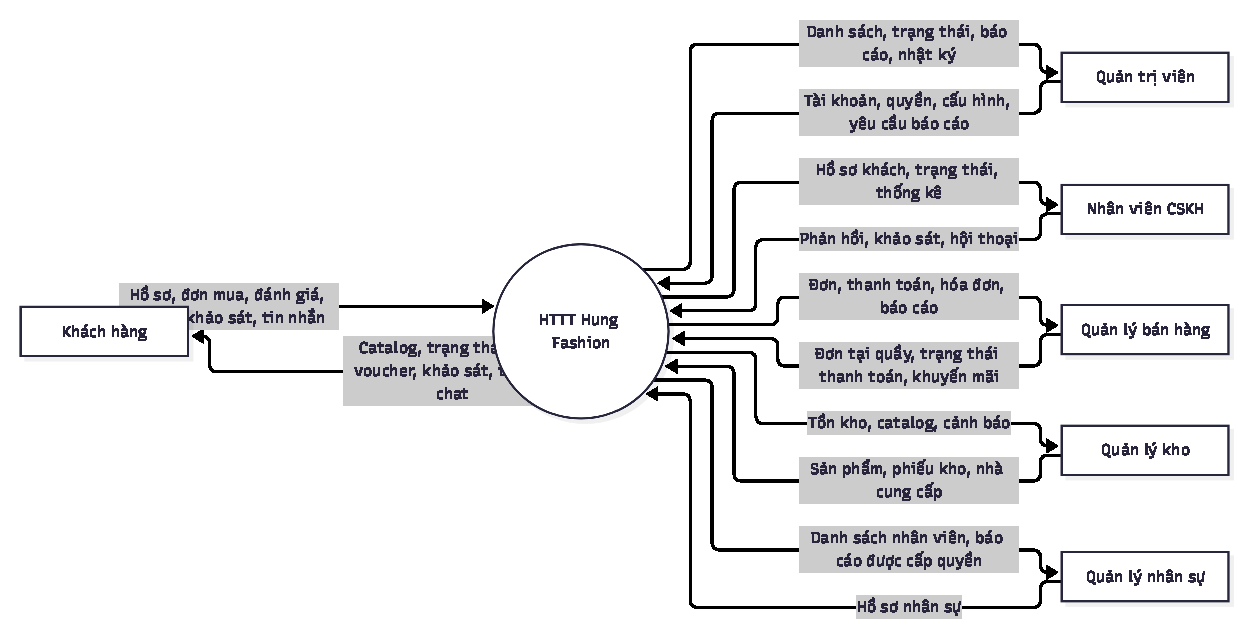
\includegraphics[width=\textwidth,height=0.68\textheight,keepaspectratio]{diagrams/02-ngu-canh.pdf}\caption{Sơ đồ ngữ cảnh HTTT Hung Fashion}\label{fig:context}\end{figure}}{\begin{figure}[H]\centering\fbox{\parbox[c][2cm][c]{0.82\textwidth}{\centering Cần kết xuất Mermaid từ \texttt{diagrams/02-ngu-canh.mmd}}}\caption{Sơ đồ ngữ cảnh HTTT Hung Fashion}\label{fig:context}\end{figure}}

\FloatBarrier
\clearpage
\Needspace{0.72\textheight}
\section{Sơ đồ luồng dữ liệu mức đỉnh}
Hình~\ref{fig:dfd0} trình bày năm tiến trình (1--5), năm kho dữ liệu (D1--D5), các tác nhân và luồng dữ liệu chính kết nối chúng. Đọc từ tác nhân qua tiến trình tới kho dữ liệu để theo dõi nơi dữ liệu được tiếp nhận, xử lý và lưu trữ.
\IfFileExists{diagrams/03-dfd-muc-0.pdf}{\begin{figure}[H]\centering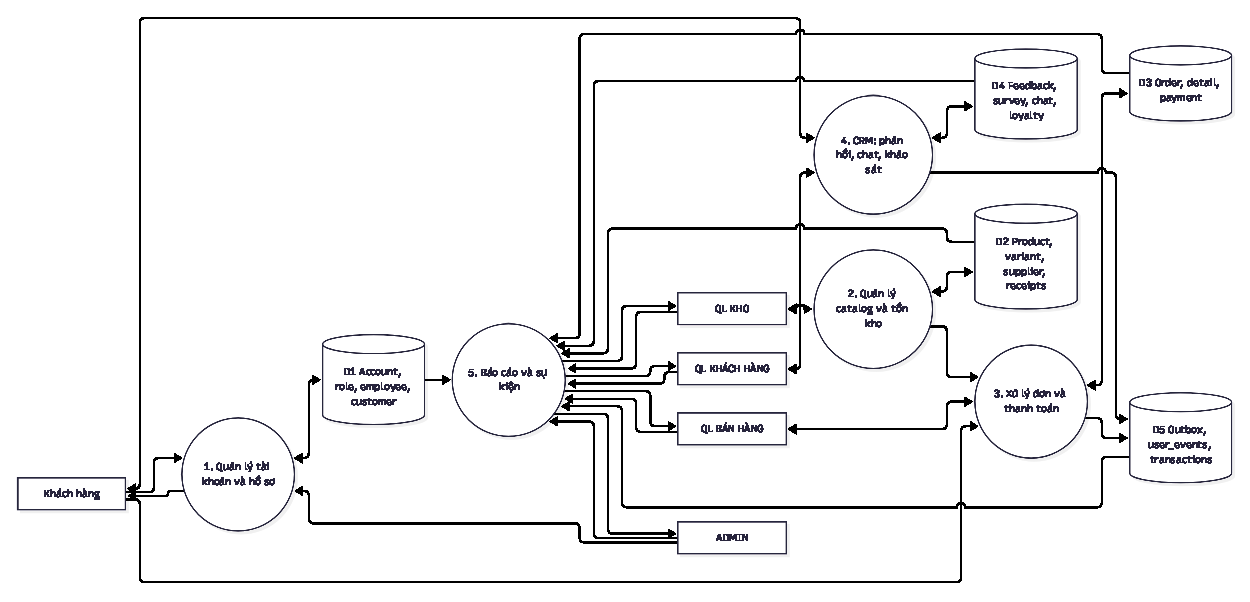
\includegraphics[width=\textwidth,height=0.68\textheight,keepaspectratio]{diagrams/03-dfd-muc-0.pdf}\caption{DFD mức đỉnh: tiến trình, tác nhân và kho dữ liệu}\label{fig:dfd0}\end{figure}}{\begin{figure}[H]\centering\fbox{\parbox[c][2cm][c]{0.82\textwidth}{\centering Cần kết xuất Mermaid từ \texttt{diagrams/03-dfd-muc-0.mmd}}}\caption{DFD mức đỉnh: tiến trình, tác nhân và kho dữ liệu}\label{fig:dfd0}\end{figure}}

\FloatBarrier
\Needspace{0.72\textheight}
\section{DFD mức 1: CRM}
Hình~\ref{fig:dfdcrm} mô tả năm quy trình CRM từ quản lý hồ sơ, tiếp nhận phản hồi và khảo sát đến ghi nhận kết quả, chat hỗ trợ; mỗi dòng nêu dữ liệu đầu vào cùng dữ liệu lưu hoặc đầu ra chính.
\begin{figure}[H]\centering\small
\begin{tabular}{|p{0.18\textwidth}|p{0.26\textwidth}|p{0.40\textwidth}|}\hline
\textbf{Tiến trình}&\textbf{Dữ liệu vào}&\textbf{Dữ liệu lưu/ra}\\\hline
4.1 Quản lý hồ sơ&Form quản lý hoặc hồ sơ khách tự cập nhật&\texttt{\detokenize{customer}}, \texttt{\detokenize{account}}, \texttt{\detokenize{interest}}, \texttt{\detokenize{customer_interest}}; danh sách và chi tiết khách\\\hline
4.2 Tiếp nhận phản hồi&Đánh giá/nội dung từ khách; trả lời và trạng thái từ CSKH&\texttt{\detokenize{feedback}}, \texttt{\detokenize{feedback_attachment}}; trạng thái và nội dung phản hồi\\\hline
4.3 Khảo sát&Tiêu chí, câu hỏi, lựa chọn, lời mời&\texttt{\detokenize{survey}}, \texttt{\detokenize{survey_question}}, \texttt{\detokenize{survey_option}}, \texttt{\detokenize{survey_invitation}}\\\hline
4.4 Thu thập kết quả&Lựa chọn/câu trả lời của khách&\texttt{\detokenize{survey_response}}, \texttt{\detokenize{survey_answer}}; bảng thống kê kết quả\\\hline
4.5 Chat hỗ trợ&Tin nhắn khách và nhân viên, metadata tệp&\texttt{\detokenize{conversation}}, \texttt{\detokenize{chat_message}}, \texttt{\detokenize{chat_message_attachment}}; event invalidation SSE\\\hline
\end{tabular}
\caption{DFD mức 1 cho nhóm chức năng CRM}\label{fig:dfdcrm}
\end{figure}

\FloatBarrier
\Needspace{0.72\textheight}
\section{DFD mức 1: đơn hàng và thanh toán}
Hình~\ref{fig:dfdorder} mô tả năm bước từ lập đơn, tính tiền và ghi nhận payment đến cập nhật trạng thái, phát sự kiện; mỗi dòng nêu đầu vào và dữ liệu lưu hoặc kết quả chính.
\begin{figure}[H]\centering\small
\begin{tabular}{|p{0.19\textwidth}|p{0.28\textwidth}|p{0.38\textwidth}|}\hline
\textbf{Tiến trình}&\textbf{Dữ liệu vào}&\textbf{Dữ liệu lưu/ra}\\\hline
3.1 Lập đơn&Khách chọn hàng/địa chỉ hoặc nhân viên tạo đơn quầy&\texttt{\detokenize{order}}, \texttt{\detokenize{order_detail}}; giảm tồn theo logic đơn\\\hline
3.2 Tính tiền&Giá, số lượng, promotion, điểm quy đổi&Tổng tiền, giảm giá, thông tin voucher và lịch sử điểm\\\hline
3.3 Ghi payment&Phương thức Cash/BankTransfer, amount&\texttt{\detokenize{payment}} với status ban đầu; QR demo token nếu cờ tính năng bật\\\hline
3.4 Cập nhật trạng thái&Yêu cầu hủy/giao hàng hoặc xác nhận thanh toán của nhân viên&Trạng thái order/payment; nghiệp vụ điểm thưởng\\\hline
3.5 Phát sự kiện&Thay đổi thanh toán đã xác nhận&\texttt{\detokenize{outbox_events}} trong transaction; relay Kafka; consumer cập nhật \texttt{\detokenize{transactions}}\\\hline
\end{tabular}
\caption{DFD mức 1 cho đơn hàng và thanh toán}\label{fig:dfdorder}
\end{figure}
